\section{Preguntas de finales}

\subsection{Baader - Marzo 2020}
\subsubsection{Procesos - Explicar diferencia entre proceso y thread y relación de este último con funciones reentrantes. Explicar qué es un árbol de procesos y cuál es su importancia}

Un proceso puede:
\begin{itemize}
\item Hacer una system call \\
\item Ejecutar en la CPU \\
\item Lanzar un proceso hijo \\
\item Realizar e/s de dispositivos \\
\item Terminar \\
\end{itemize}


Un proceso es un programa en ejecución. El proceso puede invocar tantos threads como necesite, cada thread corresponde a un único proceso. En algunas implementaciones, los recursos de los threads se distribuyen entre los recursos totales de su proceso padre, lo cual esta descripto por el árbol de procesos, y en otras pueden asignarseles recursos independientemente.

Cada proceso se refleja en un bloque de una tabla llamado Process Control Block (PCB), el cual cuenta con la información necesaria para identificar al proceso univocamente (pid) junto con data del proceso que describe el estado del proceso en el momento en que es pausado (estado, program counter, archivos abiertos, registros, stack), para asi poder reanudarlo cuando se desee y resulte transparente al proceso.

En una implementacion con threads se requiere ampliar esta implementacion de la tabla de PCB adjuntando un identificador del thread (tid), el pid del proceso al que pertenece y tambien data que permita determinar el estado de la ejecución, de la misma manera que con los procesos.

Los threads son una forma de paralelizar la ejecución de un proceso, ya sea para poder tener varias responsabilidades simultaneamente o para dividir un problema en partes y poder atacarlo mas rapidamente.

Una función reentrante es aquella que garantiza que multiples instancias de la misma pueden ejecutarse simultaneamente sin que eso provoque una falla en el sistema. Si una función fuese a ser ejecutada por distintos threads, y no hay garantías de que lo vayan a hacer de manera exclusiva, entonces esta debe ser necesariamente reentrante.

\subsubsection{Sincronización - Explicar deadlock con un dibujo y en pocas palabras}

Las $P$ son procesos y las $R$ recursos

Arcos:
\begin{itemize}
\item De $P$ a $R$, $P$ requiere $R$
\item De $R$ a $P$, $P$ adquirió $R$
\end{itemize}

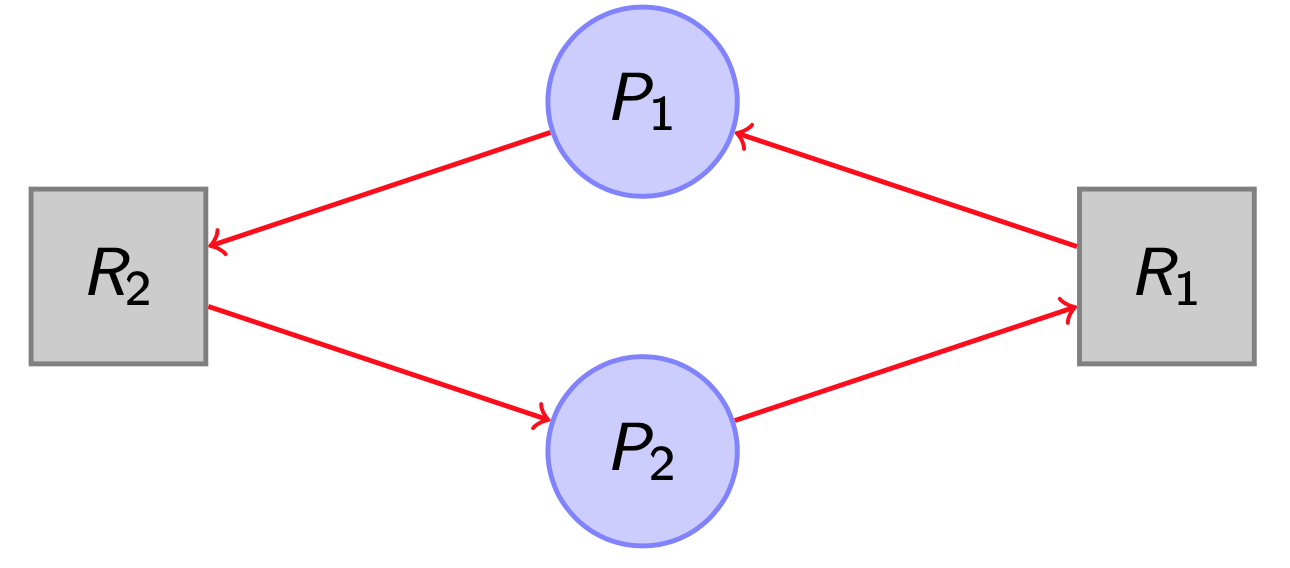
\includegraphics[width=0.6\textwidth]{imagenes/deadlock}

\subsubsection{Administración de E/S - ¿Por qué los algoritmos de scheduling se miden en cilindros? ¿Está bien? ¿Por qué? Explicar SAN}
Se llama \textit{seek time} al tiempo que tarda el brazo de un HDD en transportar los cabezales al cilindro correspondiente. El tiempo de accesso depende mayormente del \textit{seek time} y de la latencia de rotación.

Los algoritmos de scheduling de E/S definen de qué manera se moverá el brazo del disco lo cual determina el orden en que se atenderán los pedidos, en función del número de cilindro de cada uno. Cuanta más distancia recorra el brazo para cumplir los pedidos, mayor será el \textit{seek time} y más tardará en completarlos. Se miden en cilindros porque es la unidad de distancia del movimiento del brazo, cuanto mejor estén ordenados los pedidos, menos cilindros el brazo tendrá que recorrer para servirlos y mejor será el tiempo hasta completarlos.

SAN significa Storage Area Network. Se trata de tener el almacenamiento en la red, pero una red especial, donde los protocolos son específicos para este tipo de datos (son de más bajo nivel). 

El problema de tener Network Attached Storage (NAS) es que las operaciones consumen ancho de banda repercutiendo en la comunicación de la red.

\subsubsection{Seguridad - Explicar qué es una función de hash segura y ejemplificar dos usos en un sistema operativo. - comparar DAC y MAC}

Una función de hash segura es aquella que tiene muy baja probabilidad de generar colisiones y que sea muy difícil de revertir, es decir, sabiendo $y$ encontrar $x$ siendo $f(x) = y$, con $f$ la función de hash.

Discretionary Access Control (DAC): El acceso se controla basandose en las identidades de los usuarios y grupos. Se puede implementar con una matriz donde se almacena para cada sujeto, los distintos permisos sobre cada objeto. Los atributos de seguridad se definen explicitamente (se puede hacer solamente lo que está especificado). Es el usuario dueño del archivo quien determina quiénes tienen acceso al mismo.

Mandatory Access Control (MAC): Cada sujeto tiene un grado (se suele manejar el concepto de label). Los objetos heredan el grado/label del último sujeto que los modificó. Un sujeto sólo puede acceder a objetos de grado igual o menor que el suyo.

\subsubsection{Filesystems - Explicar journaling en ext3. ¿Qué problema resuelve?}

Cuando el sistema quiere realizar una transacción, en lugar de realizarla inmediatamente, se la escribe en el \textit{journal}. A esto se lo llama realizar un \textit{commit}. Un vez hecho el \textit{commit}, se devuelve el control al proceso usuario mientras el filesystem hace el replay de los commits registrados.

Este otro proceso mantiene un puntero que indica la operación dentro del commit que se está llevando a cabo, el cual va moviendo a medida que va satisfaciendo las operaciones y con ellas, los commits. Este algoritmo permite que ante una falla completa del sistema que requiera un reinicio, se pueda consultar el \textit{journal} para asi reestablecer el sistema mediante el puntero, y continuar con la operación que habia quedado pendiente, asi como con el resto de los commits que aún no habían sido ejecutados.

\subsection{Baader - Diciembre 2019}
\subsubsection{Procesos - Una página es compartida por dos procesos. Puede suceder que para un proceso sea de sólo lectura mientras que el otro tenga permitida la escritura?}

\subsubsection{Sincronización - ¿Cómo podrías sincronizar dos procesos usando IPC? ¿Cuál es la diferencia entre Spin locks y semáforos? ¿Cuándo utilizaría cada uno?}

Podrías sincronizarlos usando:
\begin{itemize}
\item Memoria compartida \\
\item Algún otro recurso compartido (archivo, base de datos) \\
\item Pasaje de mensaje
\end{itemize}

Los Spin Locks hacen busy waiting, los semáforos no. 

Además, no existe un orden cuando se utiliza un Spin Lock: los procesos continúan compitiendo por entrar a la zona crítica y se puede dar que un proceso nunca pueda acceder ya que el mecanismo se basa en simplemente consultar todos simultáneamente. En cambio, mediante semáforos, los procesos entran en waiting (no hacen espera activa sino que se duermen, esto requiere acceso al kernel) y se añaden a una cola para luego ser desencolados en el momento en que se pueda liberar el lock para dejar entrar a otro (hacer el signal).

\subsubsection{Seguridad - Describir setUID y buffer overflow y un ataque que incluya ambos}

setUID es un atributo booleano que tienen los archivos que, cuando esta activado, permite que el proceso corra esa rutina con el permiso del owner del archivo. Esto permite realizar distintas acciones que requieren permisos mas elevados, de una manera controlada ya que solo se ejecuta con ese permiso la rutina descripta por el archivo y luego se revocan.

Por ejemplo, si tuviera la necesidad de modificar un archivo con hashes de contraseñas de usuarios, necesitaría permisos de administrador. Gracias a setUID, puede crearse una rutina que modifique ese archivo de la manera controlada en que el diseñador del sistema operativo desee, permitiendo a cualquier proceso invocarla.

Un buffer overflow es un tipo de inyección de código. Es cuando un atacante se aprovecha de un programa que corre una función insegura en términos de tamaños de buffers, como lo es strcpy() que copia dentro del buffer hasta encontrar un byte NULL, haciendo que se escriba tanto contenido en el buffer en memoria que lo sobrepase y sobreescriba memoria por fuera del buffer. De esta forma se pueden sobreescribir las variables que estan almacenadas en el stack y si se sobreescribe un poco mas, se puede modificar la dirección de retorno, logrando que una vez finalizada la función se redirija la ejecución a una porción de memoria controlada por el atacante. De esta forma se termina ejecutando ese código controlado por el atacante, con el ID efectivo del proceso.

Un ataque posible sería realizar un buffer overflow sobre una rutina con setUID activado, y de esta forma conseguir ejecutar código controlado por el atacante, con el UID efectivo del owner del archivo.

\subsubsection{E/S - ¿Cómo afectan los dispositivos de memoria de estado sólido a los algoritmos de scheduler de E/S? Definir Storage Area Network (SAN)}

Los dispositivos de memoria de estado sólido no tienen problema para leer una posición aleatoria de la memoria como ocurre con los HDD, por lo que suele utilizarse una política FCFS, pero tienen otro problema ocasionado por las características de los semiconductores NAND que los componen: pueden ser leidos y escritos de a páginas (similar a los sectores en HDD) pero no pueden ser sobreescritos. Para lograr eso se deben borrar, lo cual tarda más que escribir y mucho más que leer, y luego escribir. Además, el borrado se hace de a bloques (que tienen varias paginas de tamaño).

Para evitar tener que borrar y así poder ahorrarse el tiempo de hacerlo, lo que se hace es escribir en otra pagina y marcar la vieja como invalida en la FTL (Flash Translation Layer). Cuando ya no hay paginas libres, se busca un bloque inválido (todas las páginas inválidas) para ser borrado y luego escrito. Sin embargo, puede ocurrir que no existan bloques inválidos, pero si bloques con algunas páginas invalidas que no se pueden borrar individualmente porque el borrado se hace de a bloques. Como la lectura y escritura sí es de a páginas, se podrían leer las paginas validas de un bloque y escribirlas en otro para así salvar esas paginas y poder borrar ese bloque (textit{garbage collection}). Pero como el problema nace de que el disco este lleno, no hay un lugar a donde salvar esas páginas, por lo que se hace textit{over-provisioning}: se deja siempre un porcentaje del disco libre para poder salvar esas páginas hasta liberar los bloques.

También ocurre que estos dispositivos se gastan luego de ser borrados muchas veces, por lo que la controladora trata de balancear dónde guarda fisicamente los datos en relación a que tan seguidos son borrados los bloques que los contienen (textit{wear leveling}).

Estas características de los dispositívos de memoria de estado sólido provocan que se utilize FCFS para requests de lectura pero no para escritura ya que varían de una manera no uniforme que depende de qué tan lleno esté el disco (ahí entran en acción textit{garbage collection} y textit{over-provisioning}).

Una Storage Area Network es una red independiente de alta velocidad que conecta múltiples servidores con una red de dispositivos de almacenamiento. Cada servidor puede acceder a los dispositivos como si fuese un disco conectado directamente al servidor. Esto simplifica el mantenimiento de los dispositivos de almacenamiento porque permite que estén todos centralizados físicamente en un lugar, independientemente de donde estén los servidores. También permite cambiar el programa que se corre en cada servidor y que aun así pueda acceder a los datos que necesita.

\subsubsection{Describir page fault. ¿Qué pasa cuando salta un page fault cuando una página no está en memoria? Describir el proceso.}

Las páginas de un proceso que no están en memoria o que no son accesibles por el mismo, son marcadas en la page table como inválidas. Cuando el proceso intenta acceder a una página inválida se produce un page fault. El hardware de paginado detecta el bit de inválido al intentar traducir la dirección de memoria y le causa una trap al sistema operativo.

Cuando la página en cuestión no está en memoria ocurre lo siguiente:
\begin{enumerate}
\item Se toma un frame libre (si no hay se aplicará la politica de desalojo que corresponda) \\
\item Se lee la página del almacenamiento secundario dentro del frame asignado \\
\item Se actualiza la page table con la nueva dirección de memoria de la página \\
\item Se reinicia la instrucción
\end{enumerate}

\subsubsection{¿Cómo funciona protección en paginado?}
La protección en paginado se logra a través de bits de protección asociados a cada frame, generalmente dentro de la tabla de páginas. Un bit puede servir para indicar que un frame es de lectura-escritura o de sólo lectura para ese proceso.

Al mismo momento que la dirección física está siendo computada, pueden chequearse los bits de protección para asegurarse de no estar tratando de escribir un frame de sólo lectura. Si se intentara escribir en un frame de sólo lectura, se levantaría una trap al sistema operativo. Lo mismo podría idearse para distintos tipos de acceso que quieran definirse, como por ejemplo sólo ejecución, agregando más bits de protección, permitiendo distintas combinaciones entre ellos.

También se agrega un bit a la entrada de la tabla de páginas indicando si la página es válida o inválida: si es válida es porque está en el espacio lógico de direcciones.